% !TEX root = ../thesis.tex
\todofr{WIP April 15: uncomment as you go, write story on paper first.}

\subsubsection{Variational inference in the exponential family}
%
The premises of both ADF and EP is performing variational inference in the exponential family $\mathcal F_{\phi}(\mathcal X)$.\add{check EP/ADF introduced} In the previous point, we showed that a target distribution $p$ could be associated with a point $\mu\in\mathcal M$ with $\mu=\E_{p}[\phi(X)]$ for some sufficient statistic $\phi$. Further, we showed that if the family is minimal and if $\mu\in\mathcal M^{\star}$, the mean parameter $\mu$ could be directly associated to a distribution in $\mathcal F_{\phi}$ with parameter $\theta$ given by $\nabla A^{\star}(\mu)$. It is therefore natural to consider this distribution $q_{\theta}$ as potentially forming a good approximation to $p$ in $\mathcal F_{\phi}(\mathcal X)$.
%
%\begin{figure}[!h]
%    \center
%	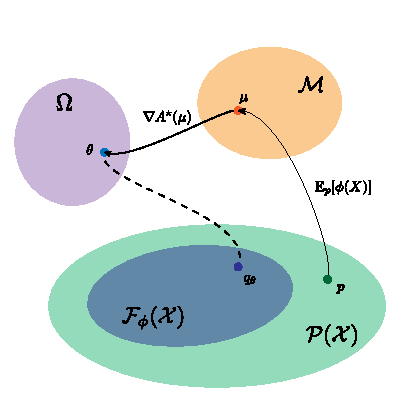
\includegraphics[width=.5\textwidth]{figures/expf/mapping2}
%\caption{blah}
%\end{figure}
This is supported by the fact that this distribution actually minimises the divergence $\KL{p,q_{\theta'}}$. Indeed, observe that
%
\eqa{
	\KL{p,q_{\theta'}} &=& \E_{p}[\log p] - \scal{\theta', \mu} + A(\theta'), \label{kldivadf}
}
%
which is a strictly convex function in $\theta'$. By definition, a parameter $\theta=\nabla A^{\star}(\mu)$ is such that $\nabla A(\theta)=\mu$ and therefore verifies the first order condition. This shows that $q_{\theta}$ minimises the divergence \eqref{kldivadf}. It is useful at this point to define a projection operator $\mathbf P_{\phi}:\mathcal P(\mathcal X) \to \mathcal F_{\phi}(\mathcal X)$ with respect to the KL divergence with
%
\eqa{	
	q \,\,=\,\, \mathbf P_{\phi}(p) &\Longleftrightarrow& q \,\,=\,\, \arg\min_{q\in\mathcal F_{\phi}(\mathcal X)} \,\, \KL{p,q}\\
	&\Longleftrightarrow& \E_{q}[\phi(X)] \,\,=\,\, \E_{p}[\phi(X)].
}
%
It will also be convenient to use the following abuse of notation: for an unnormalised distribution $p_{u}$ with normalisation constant $Z_{p_{u}}\inv$ we will write $\mathbf P_{\phi}(p_{u})$ to implicitly mean $\mathbf P_{\phi}(Z_{p_{u}}\inv p_{u})$.\\

The application of this projection operator implicitly requires the ability to perform two computations. First, it requires the ability to compute the expected value $\mu=\E_{p}[\phi(X)]$ which is typically intractable since we are in a context where we are trying to approximate $p$ for that very purpose. Then, provided we can compute $\mu$, we need to be able to recover the corresponding natural parameter by applying the inverse mapping $\nabla A^{\star}(\mu)$. We will see that by putting ourselves in a setting where the target distribution factorises into simple factors, the first requirement can be approximately met. The second requirement effectively means that we are constrained to exponential families for which computing this inverse mapping can be done explicitly or is cheap to approximate. Overwhelmingly, it is the Gaussian distribution that is considered in the literature with either a diagonal or a full covariance matrix.\add{probably add a section here on how to compute forward backward operator. Also cite lots of stuff that uses the Gaussian, if you find anything that doesn't...} 



\vspace*{2cm}\dred{gap}
Additionally, in contrast to variational Bayes, we will now consider the Kullback-Leibler divergence between the target distribution $p$ and its approximate representation $q_{\theta}\in\mathcal F_{\phi}(\mathcal X)$ i.e.:\add{make sure the contrast is clear/clarified}
%
\eqa{
	\KL{p,q_{\theta}} 
		&=& \E_{p}[\log p(X)] - \E_{p}[\log q_{\theta}(X)]\nn\\
		&=& \scal{\theta,\E_{p}[\phi(X)]} + A(\theta).
}
%
This expression is convex in $\theta$ and the first-order condition suggests minimisers in $\theta$ of the form
%
\eqa{
	\theta^{\star} &\in& \{\theta\in\Omega \mid \E_{p}[\phi(X)] = \nabla A(\theta) \}\nn\\
	&\in& \{\theta\in\Omega \mid \E_{p}[\phi(X)] = \E_{q_{\theta}}[\phi(X)]\}.\label{eq:globMM}
}
%
The condition in \eqref{eq:globMM} is called a \emph{global moment matching} condition.\add{ref to Heskes/Zoeter and co} 
Finding a parameter meeting this condition requires first the ability of computing the expected value of $\phi$ with respect to $p$ which is usually intractable.
Assuming we do find $q_{\theta^{\star}}$ minimising $\KL{p,q_{\theta}}$, we can consider it as a projection of $p$ onto $\mathcal F_{\phi}$. More generally, it is useful to define an operator $P_{\phi}:\mathcal P(\mathcal X)\to\mathcal F_{\phi}$ such that a distribution $p\in\mathcal P(\mathcal X)$ is mapped to a $q_{\theta^{\star}}\in\mathcal F_{\phi}$ verifying:
%
\eqa{
	q_{\theta^{\star}} \spe P_{\phi}[p] &\Longleftrightarrow& \E_{q_{\theta^{\star}}}[\phi(X)] \spe \E_{p}[\phi(X)].
}
%
\subsubsection{Assumed Density Filtering}

\vspace*{2cm}
In Assumed Density Filtering (ADF), we consider the problem of approximating a target distribution $p$
By contrast to MFVI, let us require the approximating distribution to be in the exponential family $\mathcal F_\phi$ associated with the sufficient statistic $\phi$. This imposes the form
\eqa{	q_\nu(x) &=& \exp\pat{\scal{\nu,\phi(x)}-A(\nu)},	}
where $\nu$ is the natural parameter of the distribution, $\phi$ the sufficient statistic of the exponential family and $A$ is the log-partition function.\footnote{We follow here the notations of \citet{wainwright08} and refer to that review for further details on the exponential family.} \\
%
%If we then look at determining the natural parameter that minimises the discrepancy $\KL{p,q_\nu}$ with
%\eqa{	\KL{p,q_\nu} &=& \E_p[\log p] - \scal{\nu,\E_p[\phi]}+A(\nu),	\nn}
%it is a convex function in $\nu$. The first order optimality condition leads to the \emph{global moment matching condition\margnote{mom.\ matching}} (using $\nabla A(\nu)=\E_{q_{\nu}}[\phi]$):
%\eqa{	\E_{q_\nu}[\phi] &=& \E_p[\phi]. 	}
%The right-hand side is intractable in general and an approximation method must be sought. At this point, we can define a projection operator $\mathcal P_\phi$ which corresponds to the projection in the KL sense onto $\mathcal F_\phi$ and is equivalently defined via the moment-matching condition:
%\eqa{		q_\nu \spe \mathcal P_\phi[p] \esp\Longleftrightarrow\esp  \E_{q_\nu}[\phi] \spe \E_p[\phi],	}
%since this condition is equivalent to minimising the KL. Note that this operator implicitly requires the ability to compute the expectation of $\phi$ with respect to $p$ as well as the ability to identify the distribution $q_{\nu}$ (i.e.: go from the mean parameter $\E_{q_{\nu}}[\phi]$ to the natural parameter $\nu$). The need to be able to perform this second step often constraints users to the Gaussian exponential family for which it is straightforward to go from the mean to the natural-parameter space.\\
%
%\textbf{Remark}: in the rest of this document, we will use the following slight abuse of notation: if $p$ is a distribution proportional to an unnormalised distribution $p_{u}$ with $p=Z_{p}\inv p_{u}$, we will also write $\mathcal P_{\phi}[p_{u}]$ to designate $\mathcal P_{\phi}[p]$. This will allow us to avoid writing explicitly normalisation constants without loss of generality.\\ 
%
%In the case where the target distribution $p$ factorises in $K$ terms $t_i$, i.e.:
%\eqa{		p(x) &=& Z_{p}\inv \prod_{i=1}^{K}t_{i}(x),\nn	}
%the \emph{assumed density filtering} (ADF)\margnote{ADF} algorithm suggests the following iteration over the natural parameter:
%\eqa{	\nu^{\text{new}} &\in& \arg\min_\nu \quad \KL{p_i,q_\nu},	\nn}
%where $p_i \propto t_i q_{\nu^{\text{old}}}$. By definition, each iteration is equivalent to a projection with:
%\eqa{	
% q_{\nu^{\text{new}}} 
%	&=& \mathcal P_\phi[ p_i],	\label{eq1 ADF}}
%except that, in the right-hand side of \eqref{eq1 ADF}, $\E_{\hat p_i}[\phi]$ is now potentially cheaper to compute or approximate. The algorithm stops when all sites have been included.\\
%
%A key issue with the ADF algorithm is that the approximating distribution depends heavily on the order in which the sites are added \citep{minka01b}. A way around this issue is the expectation propagation algorithm which, empirically, tends to outperform ADF.
%
%\subsection{\label{bg:pointEP}Expectation propagation}
%
%The expectation propagation (EP)\margnote{EP} algorithm \citep{minka01b,seeger07,gelman14}, works in much the same way as the ADF except that the sites are included in a random order and continuously. Each side is added after removing the last site approximation $\tilde t_{i}$ from the global approximation. More specifically, the core of the basic EP algorithm is formed of the following steps for each site $i$ browsed in a random order:
%\begen\itsep0
%	\item form the \emph{cavity}\margnote{cavity} by removing from $q_\nu$ the most recent approximation of the current site: $q_{\neg i} := q_\nu/\tilde t_i$,
%	\item include the true site and form the \emph{tilted distribution}\margnote{tilted} $q_i \propto q_{\neg i} t_i$,
%	\item moment-matching update: update $\nu$ s.t.\ $q_\nu\leftarrow \mathcal P_\phi[q_i]$,
%	\item store the new site approximation $\tilde t_i=q_\nu/q_{\neg i}$.
%\stopen
%The algorithm loops over the sites in a random order until convergence is reached or until the number of passes exceeds a pre-defined limit. By contrast to MFVI, convergence is not guaranteed but often observed in practice. Failure to converge is usually more telling of the selected exponential family being a poor fit to the exact posterior \citep{minka01}. Finally, EP is often empirically observed to converge much faster than MFVI and can be much better adapted to a high-dimensional setting.\footnote{For a range of applications of EP, see \url{http://research.microsoft.com/en-us/um/people/minka/papers/ep/roadmap.html}.} \\
%
%The fixed points of EP correspond to the \emph{local moment matching} conditions:
%\eqa{\E_{q_{\nu}}[\phi] &=& \E_{q_{i}}[\phi], \quad\text{for}\quad i=1,\dots,K.,\label{eq:fixedpointsep}}
%and correspond to the fixed points of the \emph{EP Energy} introduced below.
%
%\subsubsection{EP Energy}
%In the algorithm above, let us write $\tilde t_{i}(x)=\exp(\scal{\omega_{i},\phi(x)})$ the current approximation to the $i$th site. Consequently, prior to an update,
%\eqa{		q_{\neg i}(x) &=&  \exp\pat{\scal{\nu-\omega_{i},\phi(x)}}.}
%Let us define $\lambda_{i}:=\nu-\omega_{i}$ the parameter of the cavity. Then, we can write
%\eqa{ q_{i}(x) &=& t_{i}(x)\exp(\scal{\lambda_{i},\phi(x)}-A_{i}(\lambda_{i}))\nn
%	}
%where $A_{i}(\lambda_{i})$ is the log-partition function of $q_{i}$. Note also that, by definition, 
%\eqa{		\sum_{i=1}^{K}\lambda_{i} &=& (K-1)\nu.	\label{ep:condition1}}
%The \emph{EP energy} is an objective function that has the same fixed points as those corresponding to the local moment-matching condition \eqref{eq:fixedpointsep}:
%\eqa{		\mathcal E(\nu,\lambda_{1},\dots,\lambda_{K}) &:=& (K-1)A(\nu)-\sum_{i=1}^{K}A_{i}(\lambda_{i}),		}
%with $\nu$ satisfying the equality constraint \eqref{ep:condition1}. Indeed, setting the gradient of $\mathcal E$ in $\lambda_{i}$ to zero leads to precisely all the local moment matching conditions. This energy function is concave in $\lambda_{i}$, convex in $\nu$ and subject to an affine constraint. Finding EP fixed points can therefore be written as a saddle point problem:
%\eqa{		\min_{\nu}\max_{\{\lambda_{i}\}}\quad \mathcal E(\nu,\lambda_{1},\dots,\lambda_{K}), \quad \text{s.t.}\quad (K-1)\nu = \sum_{i=1}^{K}\lambda_{i}.}
%This perspective of the EP algorithm led to the so-called \emph{double-loop} algorithm of \citet{heskes03} and further theoretical considerations in \citet{opper05}. The double-loop algorithm suggests running an inner loop for the maximisation part of the saddle-point problem and alternate with an outer loop for the minimisation part. In theory, if the inner-loop is run for an infinitely long time, the algorithm can then be claimed to converge. This is however obviously impractical so that, in practice, we may suggest running the inner loop for a finite number of steps and then alternate with the outer loop. The resulting algorithm can however not be proved to converge. In some particular cases, however, it is possible to modify the algorithm so that it becomes provably convergent \citep{seeger11}.
%
%%\subsubsection{Link between EP energy and KL}
%%To get a better feel for what this EP energy represents, it is interesting to observe that both the $\KL{p,q}$ and $\KL{q,p}$ can be related to it:
%%\eqa{	
%%\KL{q,p} - \log Z_{p} &=& \mathcal E + \sum_{i=1}^{K}\KL{q,q_{i}},\nn\\
%% \KL{p,q}+\log Z_{p} &=& -\mathcal E + \sum_{i=1}^{K}\E_{p}\pac{\log {q_{i}\over q}}.\nn	}
%\subsubsection{Natural and mean parameters notations} 
%A distribution $q_{\nu}\in \mathcal F_{\phi}$ is entirely described by its natural parameter $\nu$. An alternative parametrisation is its mean parameter $\mu$ with
%\eqa{		\mu &=& \E_{q_{\nu}}[\phi].	\nn}
%%To write the EP updates in a condensed manner, it is useful to introduce the following operations that retrieve the natural and mean-parameter of a distribution $q_{\nu} \in \mathcal F_{\phi}$:
%%\eqa{	 \theta[q_{\nu}] &=& \nu\quad\text{and}\quad \mu[q_{\nu}] \spe \E_{q_{\nu}}[\phi]\nn.	}
%Under mild technical conditions, the mean and the natural parameter of $q_{\nu}$ are one to one through the gradient of the log-partition function $\nabla A$ and its inverse $\nabla A^{\star}$ with:\footnote{Here $A^{\star}$ denotes the convex conjugate of the log-partition function $A$ with $A^{\star}(\mu) = \sup_{\nu} \scal{\nu,\mu}-A(\nu)$. We refer to \citet{Rockafellar70} for more details on (sub)gradients of convex-conjugates of functions and their properties.}
%\eqa{	\nabla A^{\star}(\mu) &=& \nu.	\nn}
%With these operators, we can write the standard EP update in the following condensed form:
%\eqa{		\nu &\leftarrow&  \nabla A^{\star}[\E_{q_{i}}[\phi]].	\nn}
%Indeed, one step requires $\mu=\E_{q_{\nu}}[\phi]=\E_{q_{i}}[\phi]$ and to go from $\E_{q_{i}}[\phi]$ to $\nu$ we need to apply the operator $\nabla A^{\star}$. 
%Note that, equivalently, this update can be considered in the mean-parameter space with:
%\eqa{		\mu &\leftarrow& \E_{q_{i}}[\phi].	\nn}
%This makes a difference when damping is considered, as shown below.
%
%\subsubsection{\label{bg:pointMDEP}Damped update and mirror descent}
%To help convergence to a fixed point, the updates can be \emph{damped} 
%%[
%with a damping parameter $\gamma \in (0,1]$ (that need not be constant). If the damping is done in the natural-parameter space, the updates are modified as follows:
%%)
%\eqa{		\nu &\leftarrow&  (1-\gamma)\nu + \gamma \nabla A^{\star}\pac{\E_{q_{i}}[\phi]}.	\label{eq:ep-damped-classical}}
%It is easy to show that the corresponding update for the parameter of the local site approximation is:
%\eqa{\omega_{i} &\leftarrow& \omega_{i} + \gamma\pat{\nabla A^{\star}\pac{\E_{q_{i}}[\phi]} - \nu}.\label{sms:localupdate}}
%If the damping is done in the mean-parameter space however, the update \eqref{eq:ep-damped-classical} is modified as follows:
%\eqa{		\mu &\leftarrow& (1-\gamma)\mu + \gamma \E_{q_{i}}[\phi]
%\spe \mu + \gamma(\E_{q_{i}}[\phi] - \mu).\nn}
%This second update, when written in terms of a natural-parameter space update, corresponds to:
%\eqa{		\nu &\leftarrow& \nabla A^{\star}\pac{ \nabla A(\nu) + \gamma(\E_{q_{i}}[\phi]-\nabla A(\nu)) }.	}
%At this point, note that $\pat{\E_{q_{i}}[\phi]-\nabla A(\nu)}$ corresponds to $-\nabla_{\lambda_{i}} \mathcal E$. One can observe how this update reminds of the \emph{mirror descent algorithm}\margnote{mirror desc.} with a KL geometry. We refer to  \citet{beck03,nemirovski83} for the \emph{mirror descent algorithm} and to \citet{amari98} for the specific case of the KL geometry which yields what is know as the \emph{natural-gradient descent}\margnote{nat.\ grad.\ desc.}.\footnote{We give more details about the MDA and show the link with natural-gradient in \hyperref[app:MDA+NGD]{point~\ref*{app:MDA+NGD}}.}. \\
%%If we actually consider the MDA for this problem the update is:
%%\eqa{ \lambda_{i} &\leftarrow& \nabla A^{\star}\pac{\nabla A(\lambda_{i}) + \gamma\pat{\E_{q_{i}}[\phi]-\nabla A(\nu)} } ,	}
%%for the parameters of the cavities. This has the advantage that it can be written in terms of local stepping schemes with the shared information of the the global parameter $\nu$. 
%In line with \eqref{sms:localupdate} we can then suggest the following update for the parameters of the local site approximations:
%\eqa{\omega_{i} &\leftarrow& \nabla A^{\star}\pac{\nabla A(\omega_{i}) + \gamma\pat{\E_{q_{i}}[\phi]-\nabla A(\nu)} }.}
%This is the update considered in \citet{hasenclever16}, we will come back to it in \hyperref[sec:snep]{section~\ref*{sec:snep}}. We will show empirically how this update is more robust to noise when considering Monte Carlo estimators of $\E_{q_{i}}[\phi]$ than the natural-parameter space update \eqref{sms:localupdate}.
%
%\subsubsection{Power EP}
%We have shown that a central part of EP was the KL projection of the tilted distributions $q_{i}$ onto the exponential family. A simple extension of this framework is to consider a broader class of divergences than just the KL, the $\alpha$-divergences, which leads to the \emph{power EP} algorithm of \citet{minka04}. The basic EP algorithm is simply modified as follows:
%\begen\itsep0
%	\item form the cavity by removing from $q_\nu$ the last site approximation taken to the power $1/\beta_{i}$: $q_{\neg i}' = q_\nu/\tilde t_i^{1/\beta_{i}}$,
%	\item include the true site taken to the power $1/\beta_{i}$ and form the {tilted distribution} $q_i' \propto q_{\neg i} t_i^{1/\beta_{i}}$,
%	\item moment-matching update: update $\nu$ s.t.\ $q_\nu\leftarrow \mathcal P_\phi[q_i']$,
%	\item store the new site approximation $\tilde t_i=(q_\nu/q_{\neg i}')^{\beta_{i}}$.
%\stopen
%The rationale behind choosing the $\alpha$-divergence instead of simply the KL divergence used before is that playing with the local power $\beta_{i}$ adds a level of tuning to the framework which can help avoid overfitting, or help convergence. The precise impact of modifying the $\beta_{i}$ is however ill-understood in general but it is discussed in basic low-dimensional cases in \citet{minka05}. \\
%
%In terms of the natural-parameter space update, power EP only requires changing how the tilted distribution is constructed:
%\eqa{\omega_{i} &\leftarrow& \omega_{i} + \gamma'\pat{\nabla A^{\star}\pac{\E_{q_{i}'}[\phi]} - \nu},\nn}
%where $\gamma'=\beta_{i}\gamma$ and $q_{i}'=(t_{i}/\tilde t_{i})^{1/\beta_{i}} q$. Considering the broader framework of power EP is therefore straightforward be it for the natural or the mean-parameter space updates and adds a layer of flexibility to the framework.
